\documentclass{article}

\usepackage{ctex}
\usepackage{graphicx}
\usepackage{float}
\usepackage{datetime}
\usepackage{listings}
\usepackage{color}
\usepackage{xcolor}
\definecolor{dkgreen}{rgb}{0,0.6,0}
\definecolor{gray}{rgb}{0.5,0.5,0.5}
\definecolor{mauve}{rgb}{0.58,0,0.82}
\lstset{frame=tb,
     language=Java,
     aboveskip=3mm,
     belowskip=3mm,
     showstringspaces=false,
     columns=flexible,
     basicstyle = \ttfamily\small,
     numbers=none,
     numberstyle=\tiny\color{gray},
     keywordstyle=\color{blue},
     commentstyle=\color{dkgreen},
     stringstyle=\color{mauve},
     breaklines=true,
     breakatwhitespace=true,
     tabsize=3
}

\title{\zihao{2}\textbf{性能评测报告}}
\author{2021E8013282114\quad 吴钰轩}
\date{\today}

\begin{document}
\maketitle

\section{并发数据结构设计}
\subsection{TrainTicket类}
TrainTicket类封装的对象是某一个车次上所有座位的售票情况。\par
在该类的构造函数中,定义该车次的总座位数,车厢数和经过站台数,并且初始化一个AtomicLong类型的数组,用来记录每个座位在各个站台的售票情况,代码如下:\par
\begin{lstlisting}[ language=Java]
    public TrainTicket(int coachnum, int seatnum, int stationnum){
        seatNum = coachnum * seatnum;
        coachNum = coachnum;
        stationNum = stationnum;
        seatState = new AtomicLong[seatNum];
        for(int i = 0; i < seatNum; i ++){
            seatState[i] = new AtomicLong(0);
        }
    }
\end{lstlisting}\par
对买票操作,在购票时对座位进行上锁并分配座位,有空余座位时返回座位数,没有空余座位时返回-1。对每个座位的售出情况,采用了二进制的方式进行表示,对从departure到arrival的购票请求,将1左移(departure-arrival)位并减1,之后再左移departure位,这样得到的二进制表示中,数字0的位表示此次购票不经过该站,数字1的位表示此次购票需要经过该站。同样的,在AtomicLong的数组中也用这样的二进制数记录售票情况。在判断是否有空余座位时,遍历搜索seatState数组,将座位状态和购票状态进行按位与操作,若两者没有交集则得到结果0,此时可以在该座位上购票,并用compareAndSet更新该座位的状态。代码如下:\par
\begin{lstlisting}[ language=Java]
    public int lockForSeat(final int departure, final int arrival){
        // use binary to record which stations are used
        long passStations = (1 << (arrival - departure)) - 1;
        passStations = passStations << departure;

        // search for empty seat
        for(int i = 0; i < seatNum; i ++){
            long temp = seatState[i].get();
            // add stations to empty seat
            // spin lock
            while((temp & passStations) == 0){
                if(seatState[i].compareAndSet(temp, (temp | passStations))){
                    return i + 1;
                }
                temp = seatState[i].get();
            }
        }

        // no more seat
        return -1;
    }
\end{lstlisting}\par
对于退票操作,同样定义方法unlockForSeat,计算得到要退票的座位seatnum上的退票站台的二进制表示passStations,用compareAndSet更新seatState的新值,代码如下:\par
\begin{lstlisting}[ language=Java]
    public boolean unlockForSeat(final int seatnum, final int departure, final int arrival){

        long passStations = (1 << (arrival - departure)) - 1;
        passStations = passStations << departure;
        
        // spin lock
        while(true){
            long temp = seatState[seatnum - 1].get();
            if(seatState[seatnum - 1].compareAndSet(temp, (temp & ~passStations))){
                return true;
            }
        }
    }
\end{lstlisting}\par
最后定义查询余票的方法searchForSeat,采用按位与的方式遍历seatState数组,在查询过程中不对操作上锁,所以不能保证并发的购票和退票操作不会对查询造成影响。代码如下:\par
\begin{lstlisting}[ language=Java]
    public AtomicInteger searchForSeat(final int departure, final int arrival){
        AtomicInteger ticketNum = new AtomicInteger(0);
        long passStations = (1 << (arrival - departure)) - 1;
        passStations = passStations << departure;

        // search for tickets
        for(int i = 0; i < seatNum; i ++){
            long temp = seatState[i].get();
            if((passStations & temp) == 0){
                ticketNum.getAndIncrement();
            }
        }

        return ticketNum;
    }
\end{lstlisting}\par

\subsection{TicketingDS类}
定义ticketId表示ticket的id标号,每个ticket有唯一不同的id。定义trains数组,数组元素为TrainTicket类型,表示每一个车次的票务信息。定义ConcurrentHashMap类型的字典soldTicket记录已出售的票信息。\par
在构造函数中,根据传入参数初始化以上变量,代码如下:\par
\begin{lstlisting}[ language=Java]
    public TicketingDS(int routenum, int coachnum, int seatnum, int stationnum, int threadnum){
        trains = new TrainTicket[routenum];
        ticketId = new AtomicInteger(1);
        for(int i = 0; i < routenum; i ++){
            trains[i] = new TrainTicket(coachnum, seatnum, stationnum);
        }
        // ConcurrentHashMap for multiple situation
        soldTicket = new ConcurrentHashMap<Long, Ticket>();
    }
\end{lstlisting}\par
在购票操作中,根据车次调用对应trains[route-1]的lockForSeat方法,并记录ticket的信息,计算购得车票的车厢号和座位号,并添加到soldTicket中,代码如下:\par
\begin{lstlisting}[ language=Java]
    public Ticket buyTicket(String passenger, int route, int departure, int arrival){
        // buy ticket
        int seat = trains[route - 1].lockForSeat(departure - 1, arrival - 1);
        if(seat < 0){
            return null;
        }
        // create ticket info
        Ticket ticket  = new Ticket();
        ticket.tid = ticketId.getAndIncrement();
        ticket.passenger = passenger;
        ticket.route = route;
        ticket.departure = departure;
        ticket.arrival = arrival;
        // calculate coach and seat
        ticket.coach = ((seat - 1) / (trains[route - 1].seatNum / trains[route - 1].coachNum)) + 1;
        ticket.seat = ((seat - 1) % (trains[route - 1].seatNum / trains[route - 1].coachNum)) + 1;
        soldTicket.put(ticket.tid, ticket);
        return ticket;
    }
\end{lstlisting}\par
在退票操作中,根据票务信息重新计算出座位号,调用trains[route-1]的unlockForSeat方法删除已购得的车票,代码如下:\par
\begin{lstlisting}[ language=Java]
    public boolean refundTicket(Ticket ticket){
        // info error
        if(!soldTicket.containsKey(ticket.tid) || !(ticket == soldTicket.get(ticket.tid))){
            return false;
        }

        // calculate seat
        int seat = (ticket.coach - 1) * (trains[ticket.route - 1].seatNum / trains[ticket.route - 1].coachNum) + ticket.seat;

        // refund ticket
        if(trains[ticket.route - 1].unlockForSeat(seat, ticket.departure - 1, ticket.arrival - 1)){
            return soldTicket.remove(ticket.tid, ticket);
        }

        return false;
    }
\end{lstlisting}\par
查询操作调用trains[route-1]中的searchForSeat方法,代码如下:\par 
\begin{lstlisting}[ language=Java]
    public int inquiry(int route, int departure, int arrival){
        int restSeat = trains[route - 1].searchForSeat(departure - 1, arrival - 1).get();
        return restSeat;
    }
\end{lstlisting}\par

\newpage
\section{测试程序设计}
Test.java程序基本复制于Trace.java中的Trace类,执行过程中对各种操作总时间和总次数都做了统计,并记录了所有操作的执行时间,用于计算程序的吞吐量。下面给出在如下参数情况下的运行结果:\par 
\begin{lstlisting}[ language=Java]
    final static int[] threadnums = {1, 2, 4, 8, 16, 32, 64};
	final static int routenum = 5;
	final static int coachnum = 8;
	final static int seatnum = 100;
	final static int stationnum = 10;

	final static int testnum = 10000;
	final static int retpc = 10; // return ticket operation is 10% percent
	final static int buypc = 40; // buy ticket operation is 30% percent
	final static int inqpc = 100; //inquiry ticket operation is 60% percent
\end{lstlisting}\par
\begin{figure}[H]
    \centering
    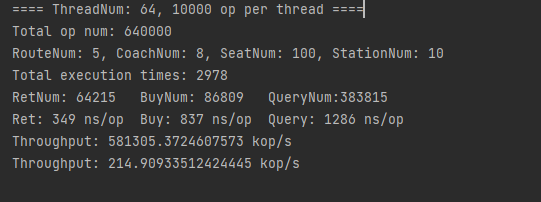
\includegraphics[width = 0.85\textwidth]{1.png}
    \caption{result}
\end{figure}

\newpage
\section{系统正确性}
\subsection{可线性化}
在TrainTicket类中,购票方法和退票方法均对所要操作的数据结构进行上锁,并采用原子操作compareAndSet()方法修改seatState数组元素的状态。退票和购票操作均可以看作是在
$$
seatState[i].compareAndSet(temp, (temp | passStations))
$$\par 
上述操作完成的时间点上退票和购票在并发数据结构中完成。lockForSeat()方法和unlockForSeat()方法中compareAndSet()所在的行就是两者的可线性化点。
\begin{figure}[H]
    \centering
    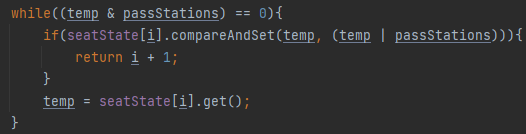
\includegraphics[width = 0.85\textwidth]{2.png}
    \caption{lockForSeat}
\end{figure}\par 
如果compareAndSet()操作没有成功,线程会不断自旋并探测,重复compareAndSet()操作。对退票方法同理。
\begin{figure}[H]
    \centering
    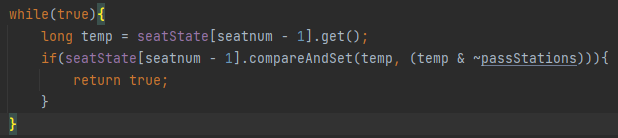
\includegraphics[width = 0.85\textwidth]{3.png}
    \caption{lockForSeat}
\end{figure}\par
\subsection{deadlock-free}
该程序是deadlock-free的,在死锁的过程中,需要两个进程相互等待,进程对请求的资源进行保持。而在本程序中,在循环等待的过程中,涉及到的操作只有:\par 
$$
seatState[i].compareAndSet(temp, (temp | passStations)
$$\par 
这样一个原子操作,并且在条件不满足时不会对temp的值进行修改,即没有对资源进行保持操作。要使得程序死锁,即说明两个进程在相互等待时,需要其中一个进程不断修改temp的值,这显然不可能出现,因为原子操作compareAndSet()一旦完成即退出循环。
\subsection{starvation-free}
由于使用了原子操作compareAndSet(),在买票和退票的进程中,进程不会在等待时不断被其他进程所打断,一旦temp修改完成即退出等待,不会出现starvation-free的现象。
\subsection{lock-free}
购票和退票操作的可线性化点均在compareAndSet()操作上,那么当temp的值没有改变时,compareAndSet()操作就可以完成,即完成买票和退票操作。能够对temp值进行修改的只有compareAndSet()操作,若所有进程都在等待状态,那么temp的值必然不变,此时任意进程都能完成compareAndSet()操作。所以,不存在所有进程均等待且temp值不断变化的情况,即至少有一个进程在同一时间能够执行。
\subsection{wait-free}
wait-free要保证每个线程在有限步骤下完成,由于进程时starvation-free,保证了每个进程都能得到执行。购票和退票操作在执行时只需要修改temp的值即可,即完成compareAndSet()操作,所以所有的进程均能在有限步内完成。

\newpage
\section{系统性能}
在route=5,coach=8,seat=100,station=10的情况下,分别对thread在各种情况下的吞吐量和执行时间进行测量。
\subsection{程序总执行时间}
在Test.java中采用System.nanoTime()测量程序执行时间,结果如下图:\par 
\begin{figure}[H]
    \centering
    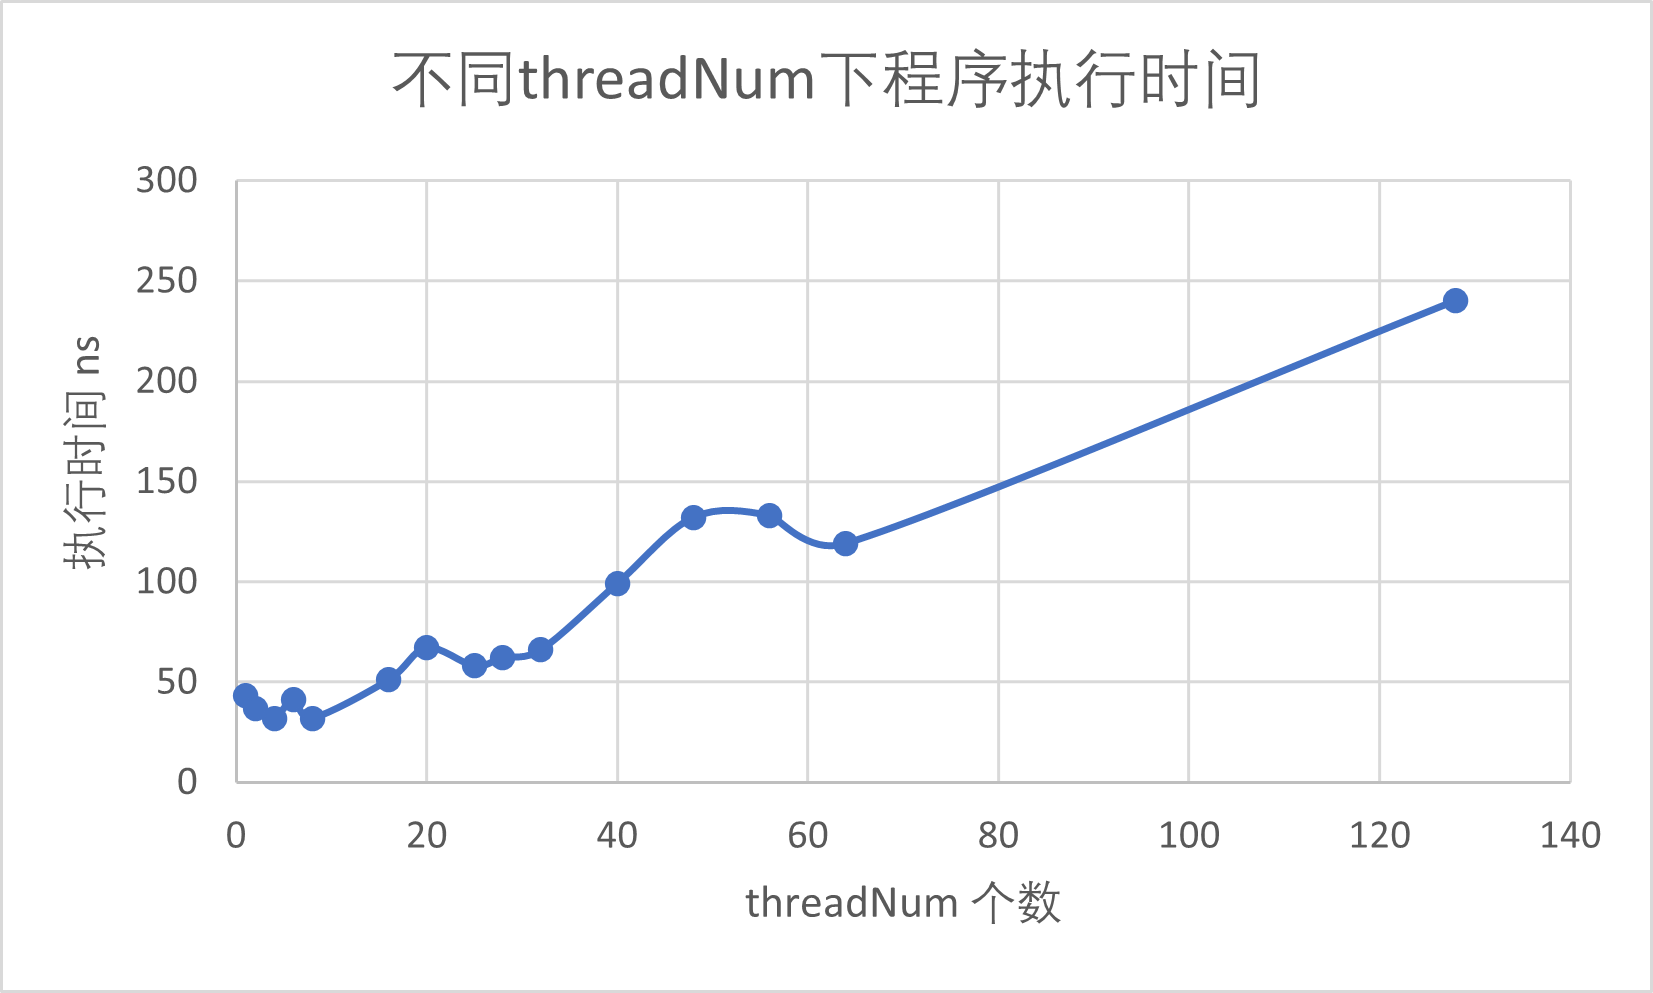
\includegraphics[width = 0.85\textwidth]{4.png}
    \caption{程序执行时间和线程数关系}
\end{figure}\par
\subsection{程序总吞吐量}
每个线程执行操作10000次,其中退票操作、购票操作和查询操作分别占10\%、30\%和60\%,用总执行操作数除以执行总时间得到程序总吞吐量,如下图:\par 
\begin{figure}[H]
    \centering
    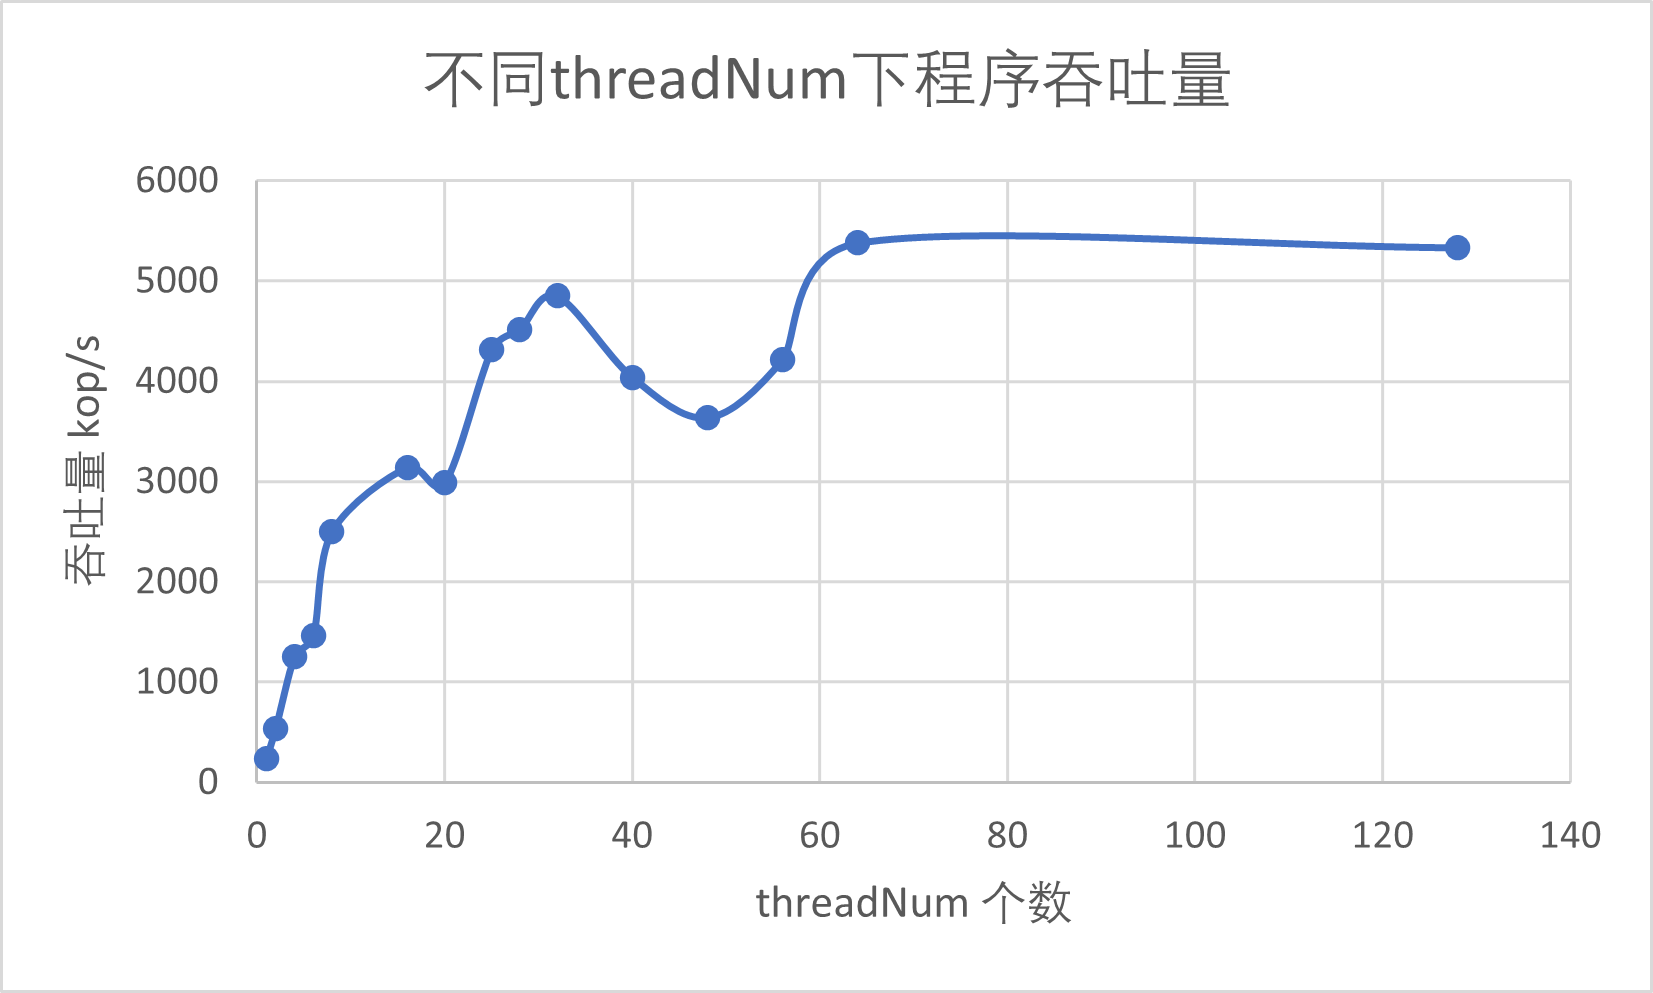
\includegraphics[width = 0.85\textwidth]{5.png}
    \caption{程序总吞吐量和线程数关系}
\end{figure}\par

\end{document}